\chapter{Theory}

Theory relevant to the spectroscopy and detection of single Ba/Ba\textsuperscript{+} in SXe matrices is discussed.  

\section{Ba/Ba\textsuperscript{+} Spectroscopy in Vacuum}

The lowest-lying energy levels in vacuum for Ba and Ba\textsuperscript{+} are shown in Fig. \ref{fig:elevs}.  For Ba, the main transition is between the ground $6s^{2}$ $^{1}$S$_{0}$ to the excited $6s6p$ $^{1}$P$_{1}$ state.  Spin{\color{red}(?)}-suppressed transitions between the P state and three metastable D states results in a decay in to a D state after about 350 excitations.  For Ba\textsuperscript{+}, two strong transitions exist between the ground $6s$ $^{2}$S$_{1/2}$ \textbf{{\color{red}is the doublet correct??}} and the $6p$ $^{2}$P$_{1/2}$ and $6p$ $^{2}$P$_{3/2}$ excited states.  Transitions to the two metastable D states are higher than for the atom, resulting in a decay into a D state after about 4 excitations.

\begin{figure}[H]
	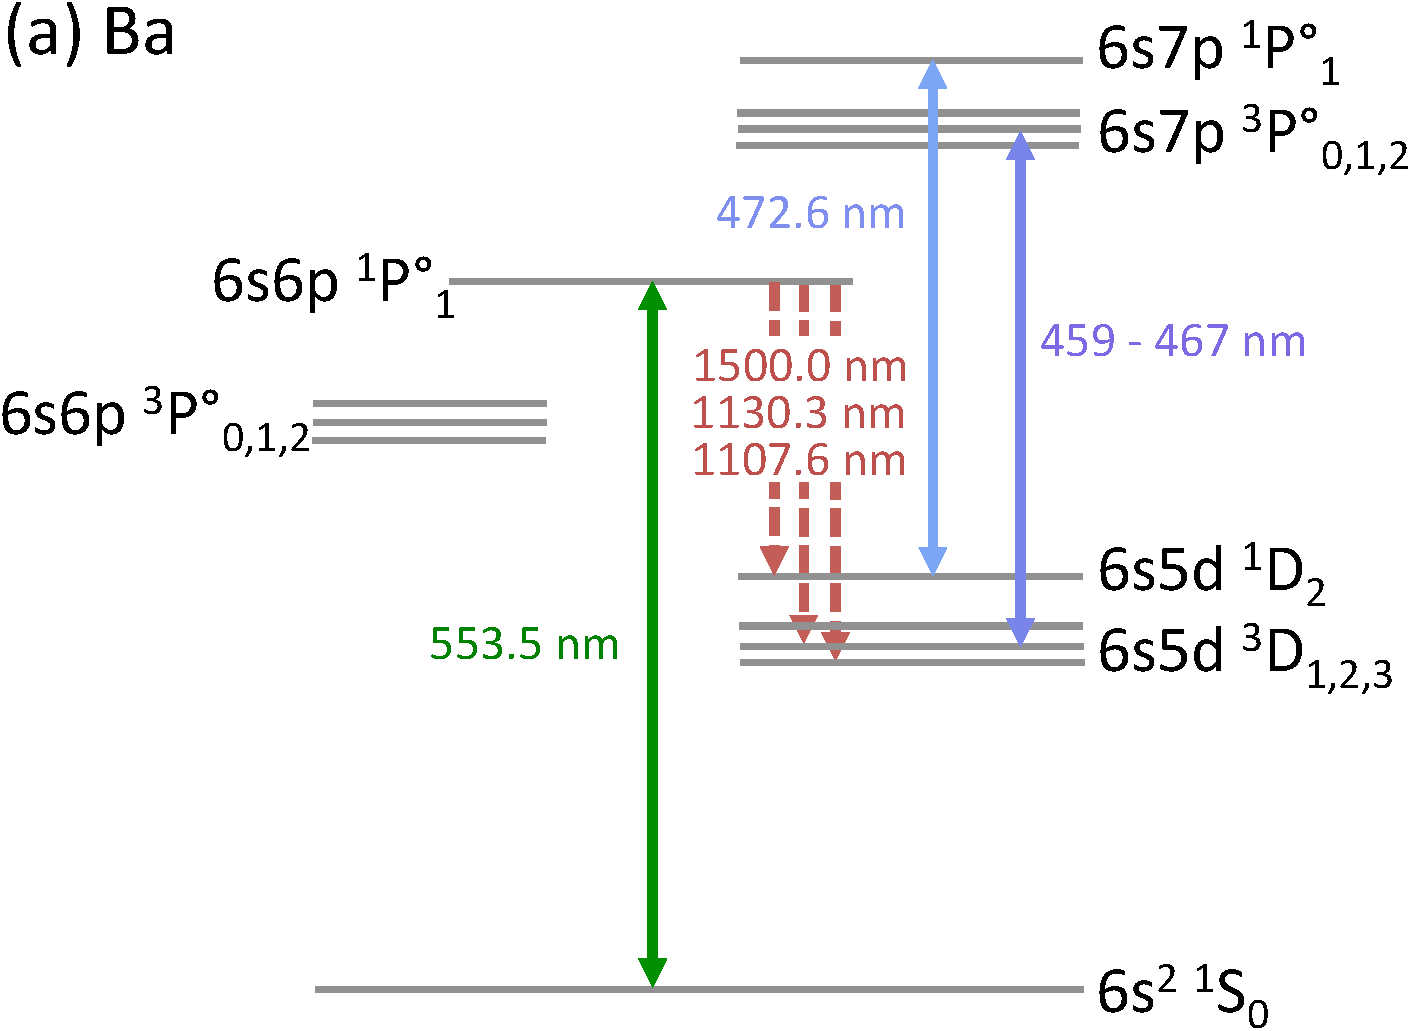
\includegraphics[width=.35\textwidth]{figures/BaLevs_atom.pdf}
	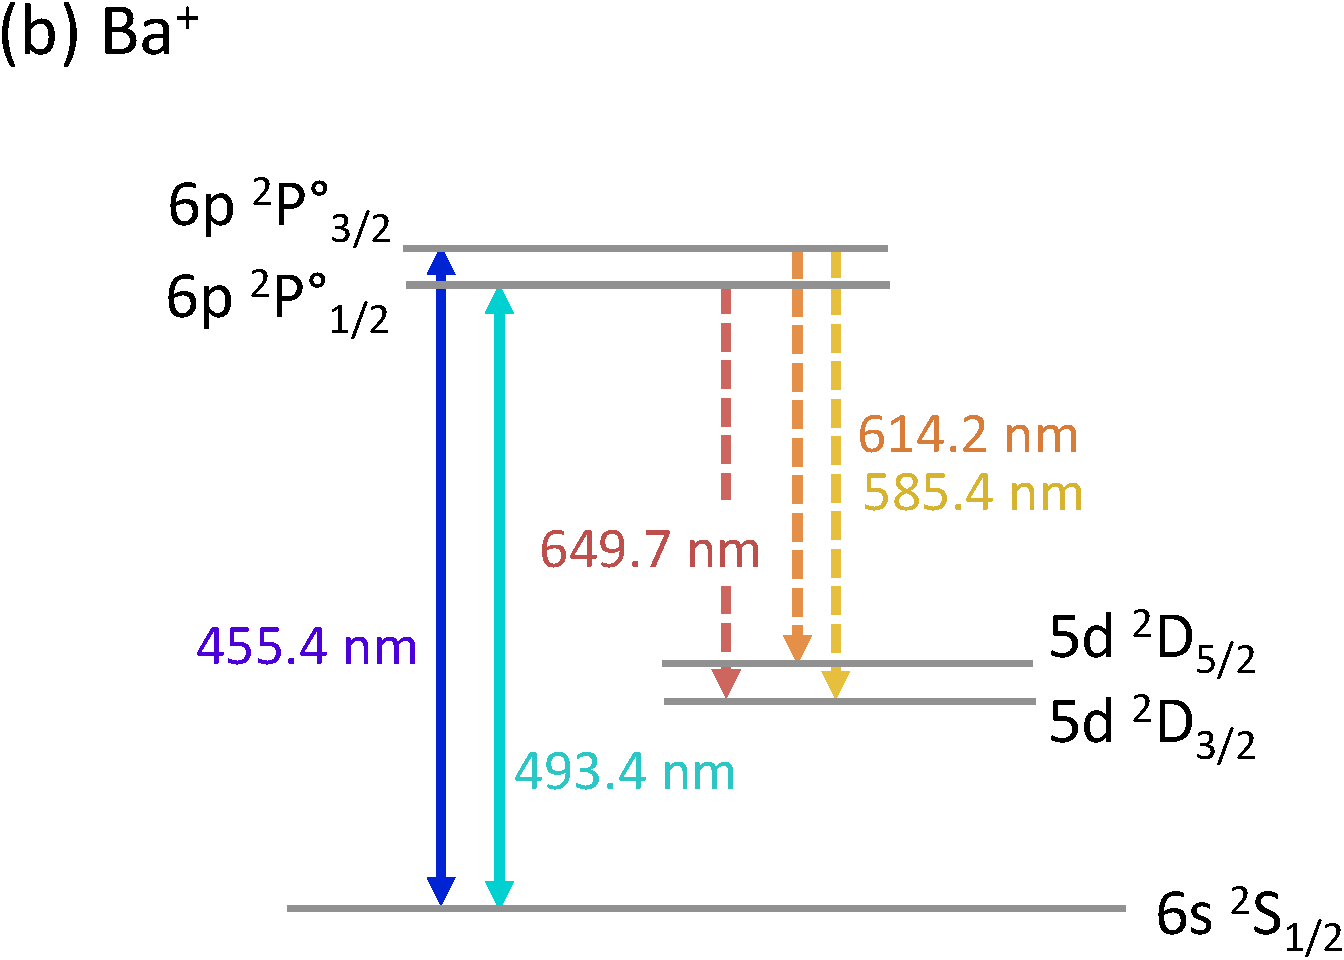
\includegraphics[width=.35\textwidth]{figures/BaLevs_ion.pdf}
	\caption{Energy level diagrams for (a) Ba and (b) Ba\textsuperscript{+} {\color{red}\textbf{Is the 2 correct in 2S1/2 in the ion?}  Get rid of high P states in Ba}}
    \label{fig:elevs}
\end{figure}

These energy levels and their transition rates are well known, and are documented in the NIST tables [ref].  Single atom/ion detection by spectroscopy generally requires lasers to provide transitions out of the metastable D states once the atom/ion decays into one of them, in addition to the main excitation laser.  For the atom, this requires three additional infrared lasers, but single atom trapping/detection in a magneto-optical trap (MOT) in [ref Ba MOT].  Single Ba\textsuperscript{+} observation requires only two lasers if the $^{2}$P$_{1/2}$ excited state is used.  This is demonstrated in [ref something that does this ... is there something?  How about the Carleton group?].

\section{Matrix Isolation Spectroscopy}

The spectroscopy of a species trapped in an inert solid matrix is called matrix isolation spectroscopy, the concept of which was pioneered around 19?? by [that one guy] [ref ... maybe [1] of ba spec].  The leading interaction between 

Studies of some systems ... (Na? Mg?)

We are of course interested in the spectroscopy of Ba and/or Ba\textsuperscript{+} in SXe matrices, and this particular system has not been studied until recently.  The first report of the spectroscopy of neutral Ba in SXe was published by our group in [ref ba spec], and conversations following this publication with ???'s group in ??? have confirmed our basic observations of the absorption spectrum og Ba in SXe.  